\documentclass[a4paper,10pt,parskip=half]{scrartcl}

\usepackage[usenames,dvipsnames]{xcolor}
\usepackage{graphicx}
\usepackage[utf8]{inputenc} %-- pour utiliser des accents en français
\usepackage{mathpazo}
\usepackage{amsmath,amssymb,amsthm} 
\usepackage[round]{natbib}
\usepackage{url}
\usepackage{xspace}
\usepackage{multirow}
\usepackage[left=20mm,top=20mm]{geometry}
\usepackage[ruled,vlined,linesnumbered]{algorithm2e}
\usepackage{subcaption}
\usepackage{booktabs}
\usepackage{colortbl}
\usepackage{hyperref}
\usepackage{boxedminipage}
\usepackage{fontawesome}
\usepackage{lastpage}
\usepackage{todonotes}
\usepackage{listings}
\usepackage{ccicons}
\usepackage{float}
\usepackage{tikz}
\usepackage[tikz]{mdframed}


\usepackage[autooneside,headsepline]{scrlayer-scrpage}
\clearpairofpagestyles
\ihead*{GEO1004.2020}
% \ohead*{Lesson 01}
% \setheadsepline{0.5pt}
\KOMAoptions{footsepline=:.25\textwidth,clines}
\cfoot{\pagemark\ of \pageref{LastPage}}


\newcommand{\ie}{ie}
\newcommand{\eg}{eg}
\newcommand{\reffig}[1]{Figure~\ref{#1}}
\newcommand{\refsec}[1]{Section~\ref{#1}}
\newcommand{\refeq}[1]{Equation~\ref{#1}}

\setcapindent{1em} %-- for captions of Figures


\renewcommand{\refname}{References \& further reading}
\renewcommand{\contentsname}{\vspace{-15mm}}

\definecolor{light-gray}{gray}{0.97}
\definecolor{myred}{RGB}{111,12,31}
\definecolor{mygreen}{RGB}{35,138,35}

\newfloat{myfloat}{thp}{lop}

\newmdenv[%
  outerlinewidth=1.5,%
  roundcorner=5pt,%
  linecolor=myred,%
  backgroundcolor=light-gray,%
  frametitle=\faExternalLink\ To read or watch,
]{link-box}

\newmdenv[%
  outerlinewidth=1.5,%
  roundcorner=5pt,%
  linecolor=mygreen,%
  backgroundcolor=light-gray,%
  frametitle=\faCog\ How does it work in practice?,
]{practice-box}

\newcommand{\lessonNumber}{Lesson 1.1}

\newtheorem{definition}{Definition}

\title{Introduction to 3D modelling of the built environment: reality, data models and data structures}


\ohead*{\lessonNumber}
\titlehead{\thispagestyle{headings}}
\author{\lessonNumber\footnote{\ccbysa\ Ken Arroyo Ohori. This work is licensed under a Creative Commons Attribution 4.0 International License (\url{http://creativecommons.org/licenses/by/4.0/})\newline(last update: \today)}}
\date{}
\begin{document}
\pagestyle{scrheadings}

\maketitle

\noindent\rule{5cm}{0.4pt}
\tableofcontents
\noindent\rule{5cm}{0.4pt}
\vspace{5mm}

%%%%%%%%%%

The 3D modelling of the built environment involves the creation, manipulation and use of 3D digital representations of real-world objects, including buildings, terrains and infrastructure.
These representations can be quite complex, since they might need to include a mix of geometric, topological and semantic information, and to do so in a manner that is both flexible (to be applicable to all the different objects that can be modelled) and consistently structured (to allow for automated processing using simple rules).
% These two requirements oppose each other in practice

In order to fulfil both of these requirements, and to be able to reuse representations in different applications, 3D modelling is done through a series of abstractions of the real world, each working at a different abstraction level.
For instance, a typical high-level abstraction could divide the world into discrete objects (\eg\ individual buildings or plots of land), whereas a lower-level abstraction could divide each surface of a wall into triangles (\ie\ meshing) while satisfying certain characteristics.
Each abstraction is thus an engineered partial solution to a complex modelling problem, which comes with its own technical choices, advantages and disadvantages, and applications for which it is suitable (or not).

For example, a 3D city model can be stored in a \texttt{.json} file where its entities are structured according to the CityJSON data model, with geometries represented as solids, and where each semantic surface is a triangulated mesh.
Alternatively, we can have a classified point cloud of the same city stored in an indexed series of \texttt{.las} files representing tiles.
Out of these two representations, the point cloud can be easily used as base elevation data or for many visualisation-based operations with comparatively little processing, but even simple spatial analysis operations (\eg\ counting the number of buildings or computing their volume) can be very complex.
On the other hand, the 3D city model could be used for complex spatial analysis operations (\eg\ wind and solar radiance simulations; \reffig{fig:applications}), but some objects that are present in the real-world (\eg\ trees and fences) might be omitted in the model.

\begin{figure}
\centering
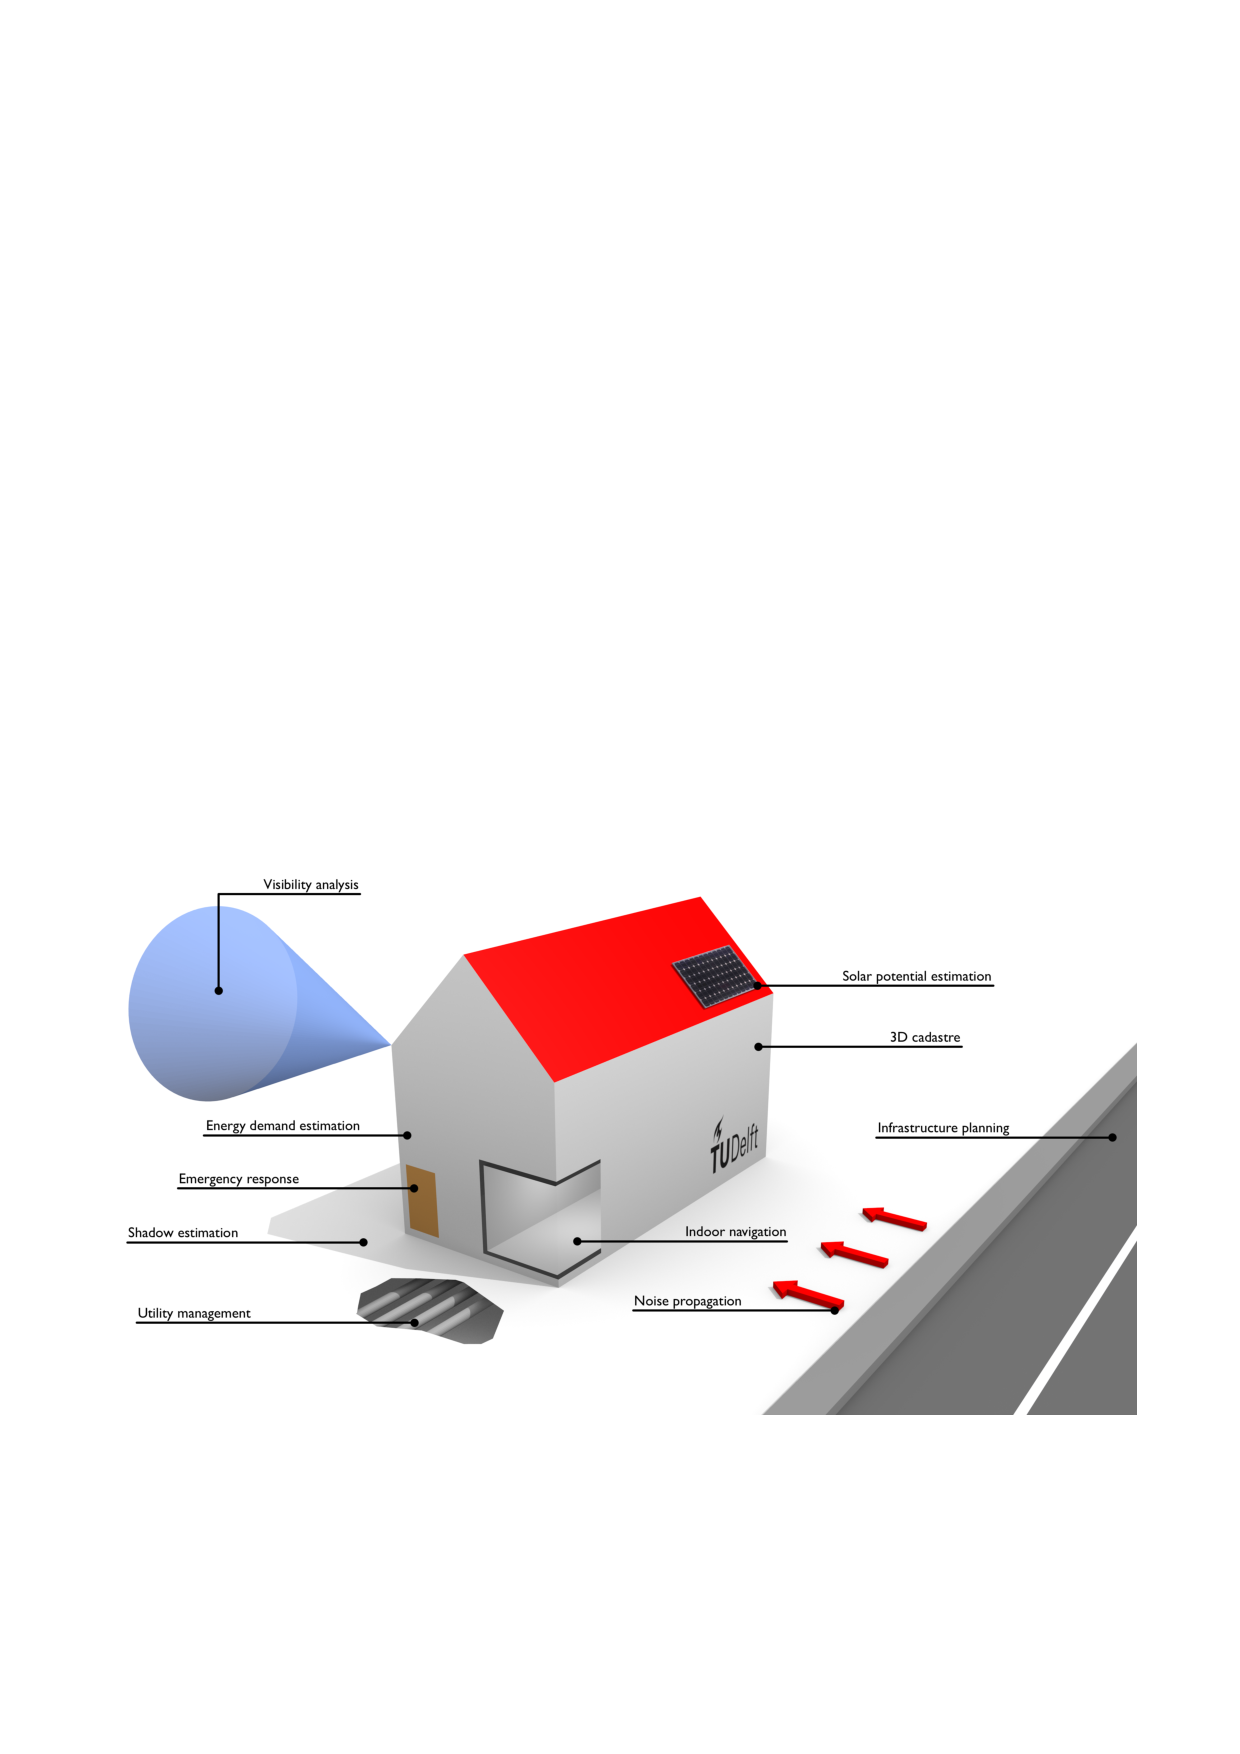
\includegraphics[width=\linewidth]{figs/applications.pdf}
\caption{Some typical applications of 3D city models~\citep{Biljecki15a}.}%
\label{fig:applications}
\end{figure}

\section{Spatial concepts}

In order to conceptualise and structure the real world, 3D models of the built environment rely on some common spatial concepts.
Some of the most common ones are:

\begin{description}

\item[The geoinformation chain]
From a practical perspective, a common way to consider how space is structured is based on the usual steps in the geoinformation chain (or pipeline).
This considers that one starts from the acquisition of data, either through traditional measurements (using anything from a tape measure to a total station) or using a variety of sensing technologies, including active methods using the reflections of electromagnetic waves (\eg\ all forms of lidar and radar) and vibrations (\eg\ underwater echo sounding and seismic methods), as well as passive methods (\eg\ digital images using any spectrum).

These `raw' measurements are then used to create simple primitives (\eg\ the points in a point cloud or the plane equation of a wall), and these are then further processed and assembled to create more complex 3D objects.

For instance, a typical process can go from a set of lidar full waveforms to a point cloud by deciding on appropriate return power thresholds, then to a series of meshes by reconstructing surfaces and fitting planes, and finally to a 3D city model with semantic surfaces by classifying and assembling the surfaces into 3D objects.
In every step of such a process, there is certain amount of information loss, but (ideally) the information that remains is more structured and meaningful.

\item[Objects and fields]
From a theoretical GIS standpoint, the typical way to conceptualise space recognises two ways of looking at the world: \emph{objects} and \emph{fields}.
The objects view considers that space is empty and is populated by discrete objects.
In many cases, this results in an approach where objects are modelled individually (\eg\ a building modelled as a set of surfaces), although they can also be aggregated or generalised into (\eg\ a set of adjacent buildings with the same height modelled as a single block).

By contrast, the fields view considers that there are certain attributes that fill space and have a value everywhere in it.
The typical examples are physical characteristics, such as the elevation of a terrain, the temperature or the wind speed.
Since we generally cannot know or store the values of fields in every possible location, of which there might be infinitely many, the standard approach is to mathematically model an approximation (\eg\ elevation modelled as an interpolated set of points).

\item[Euclidean, Cartesian and point set geometry]
When we model objects mathematically, we often rely on abstract geometric shapes, such as point, lines and planes.
The simplest mathematical descriptions for these are based on \emph{Euclidean geometry}.
Euclidean geometry starts from a small set of geometric axioms considered to be intuitively obvious (\reffig{fig:line}).
Using these axioms, it is possible to construct more complex objects (\eg\ a triangle covering the area between three points) and to define properties, such as relative distances, angles and areas.
However, objects in Euclidean geometry do not have an absolute position in space.

\begin{figure}
\centering
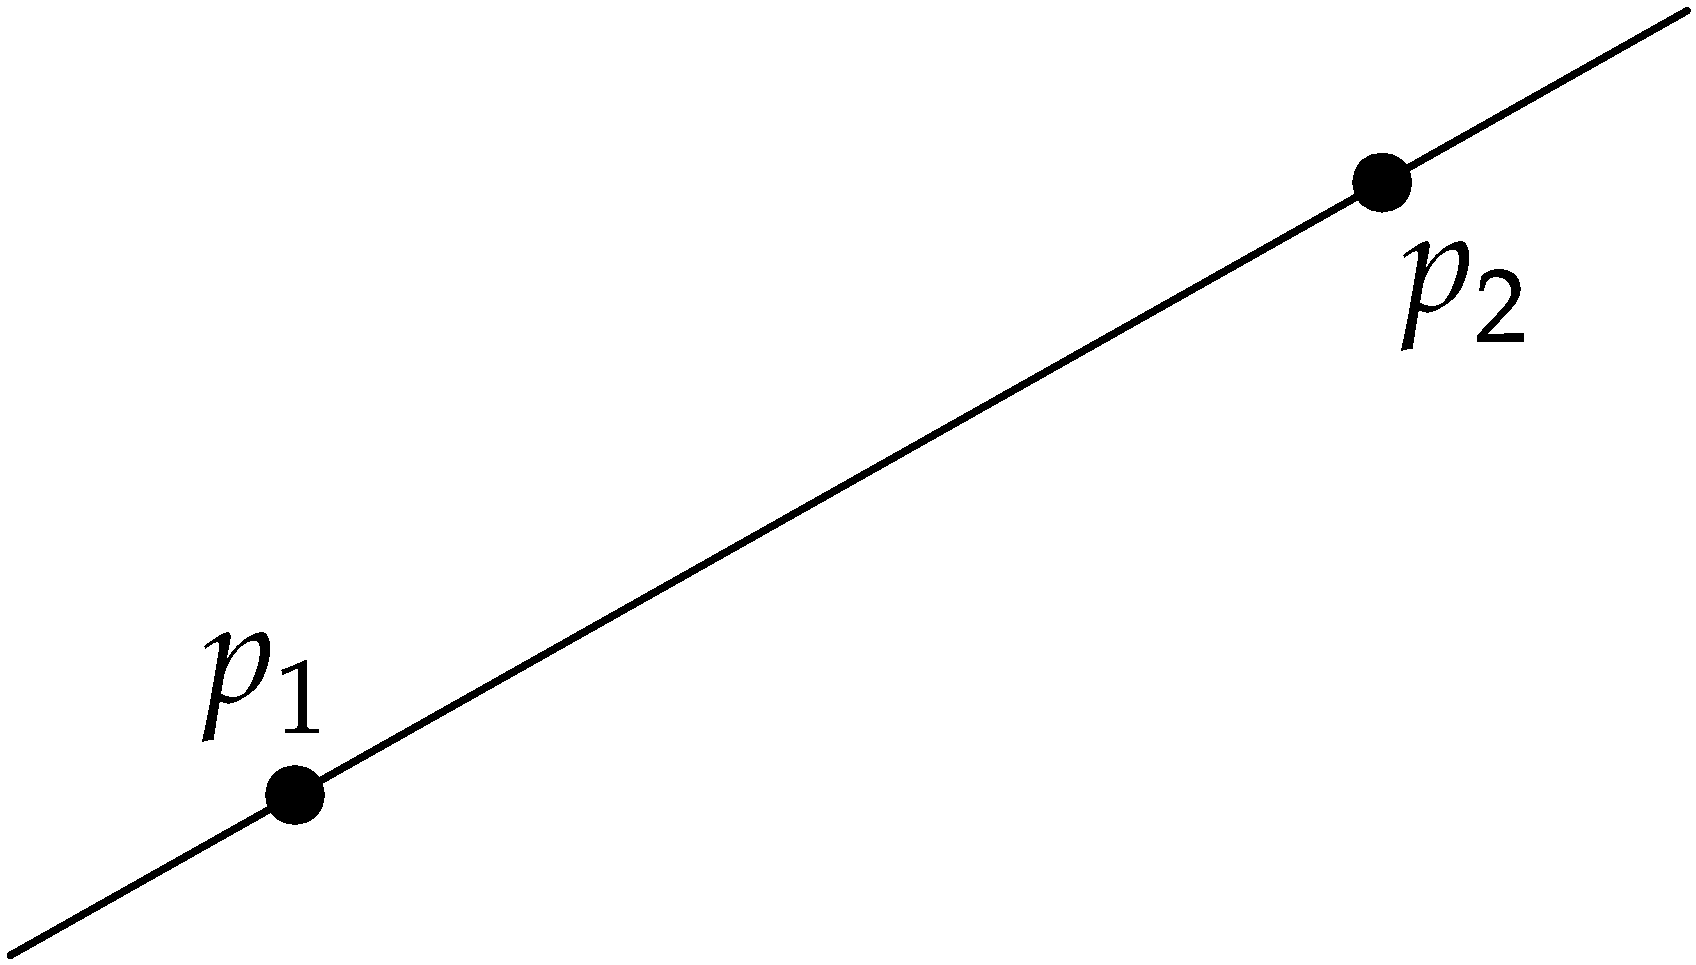
\includegraphics[width=0.3\linewidth]{figs/line.pdf}
\caption{Since there is exactly one line that passes through any pair of points, two points can be used to describe a line in Euclidean geometry.}%
\label{fig:line}
\end{figure}

Where this notion is required, analytic or \emph{Cartesian geometry} adds the concept of coordinates to the objects of Euclidean geometry, which makes it possible to uniquely describe the absolute location of a point (\reffig{fig:point}), the length of a line or the angle between two lines.
This analytic description also makes it possible using algebra to compute the exact value of some properties, such as the distance between two points (as described by their coordinates).

\begin{figure}
\centering
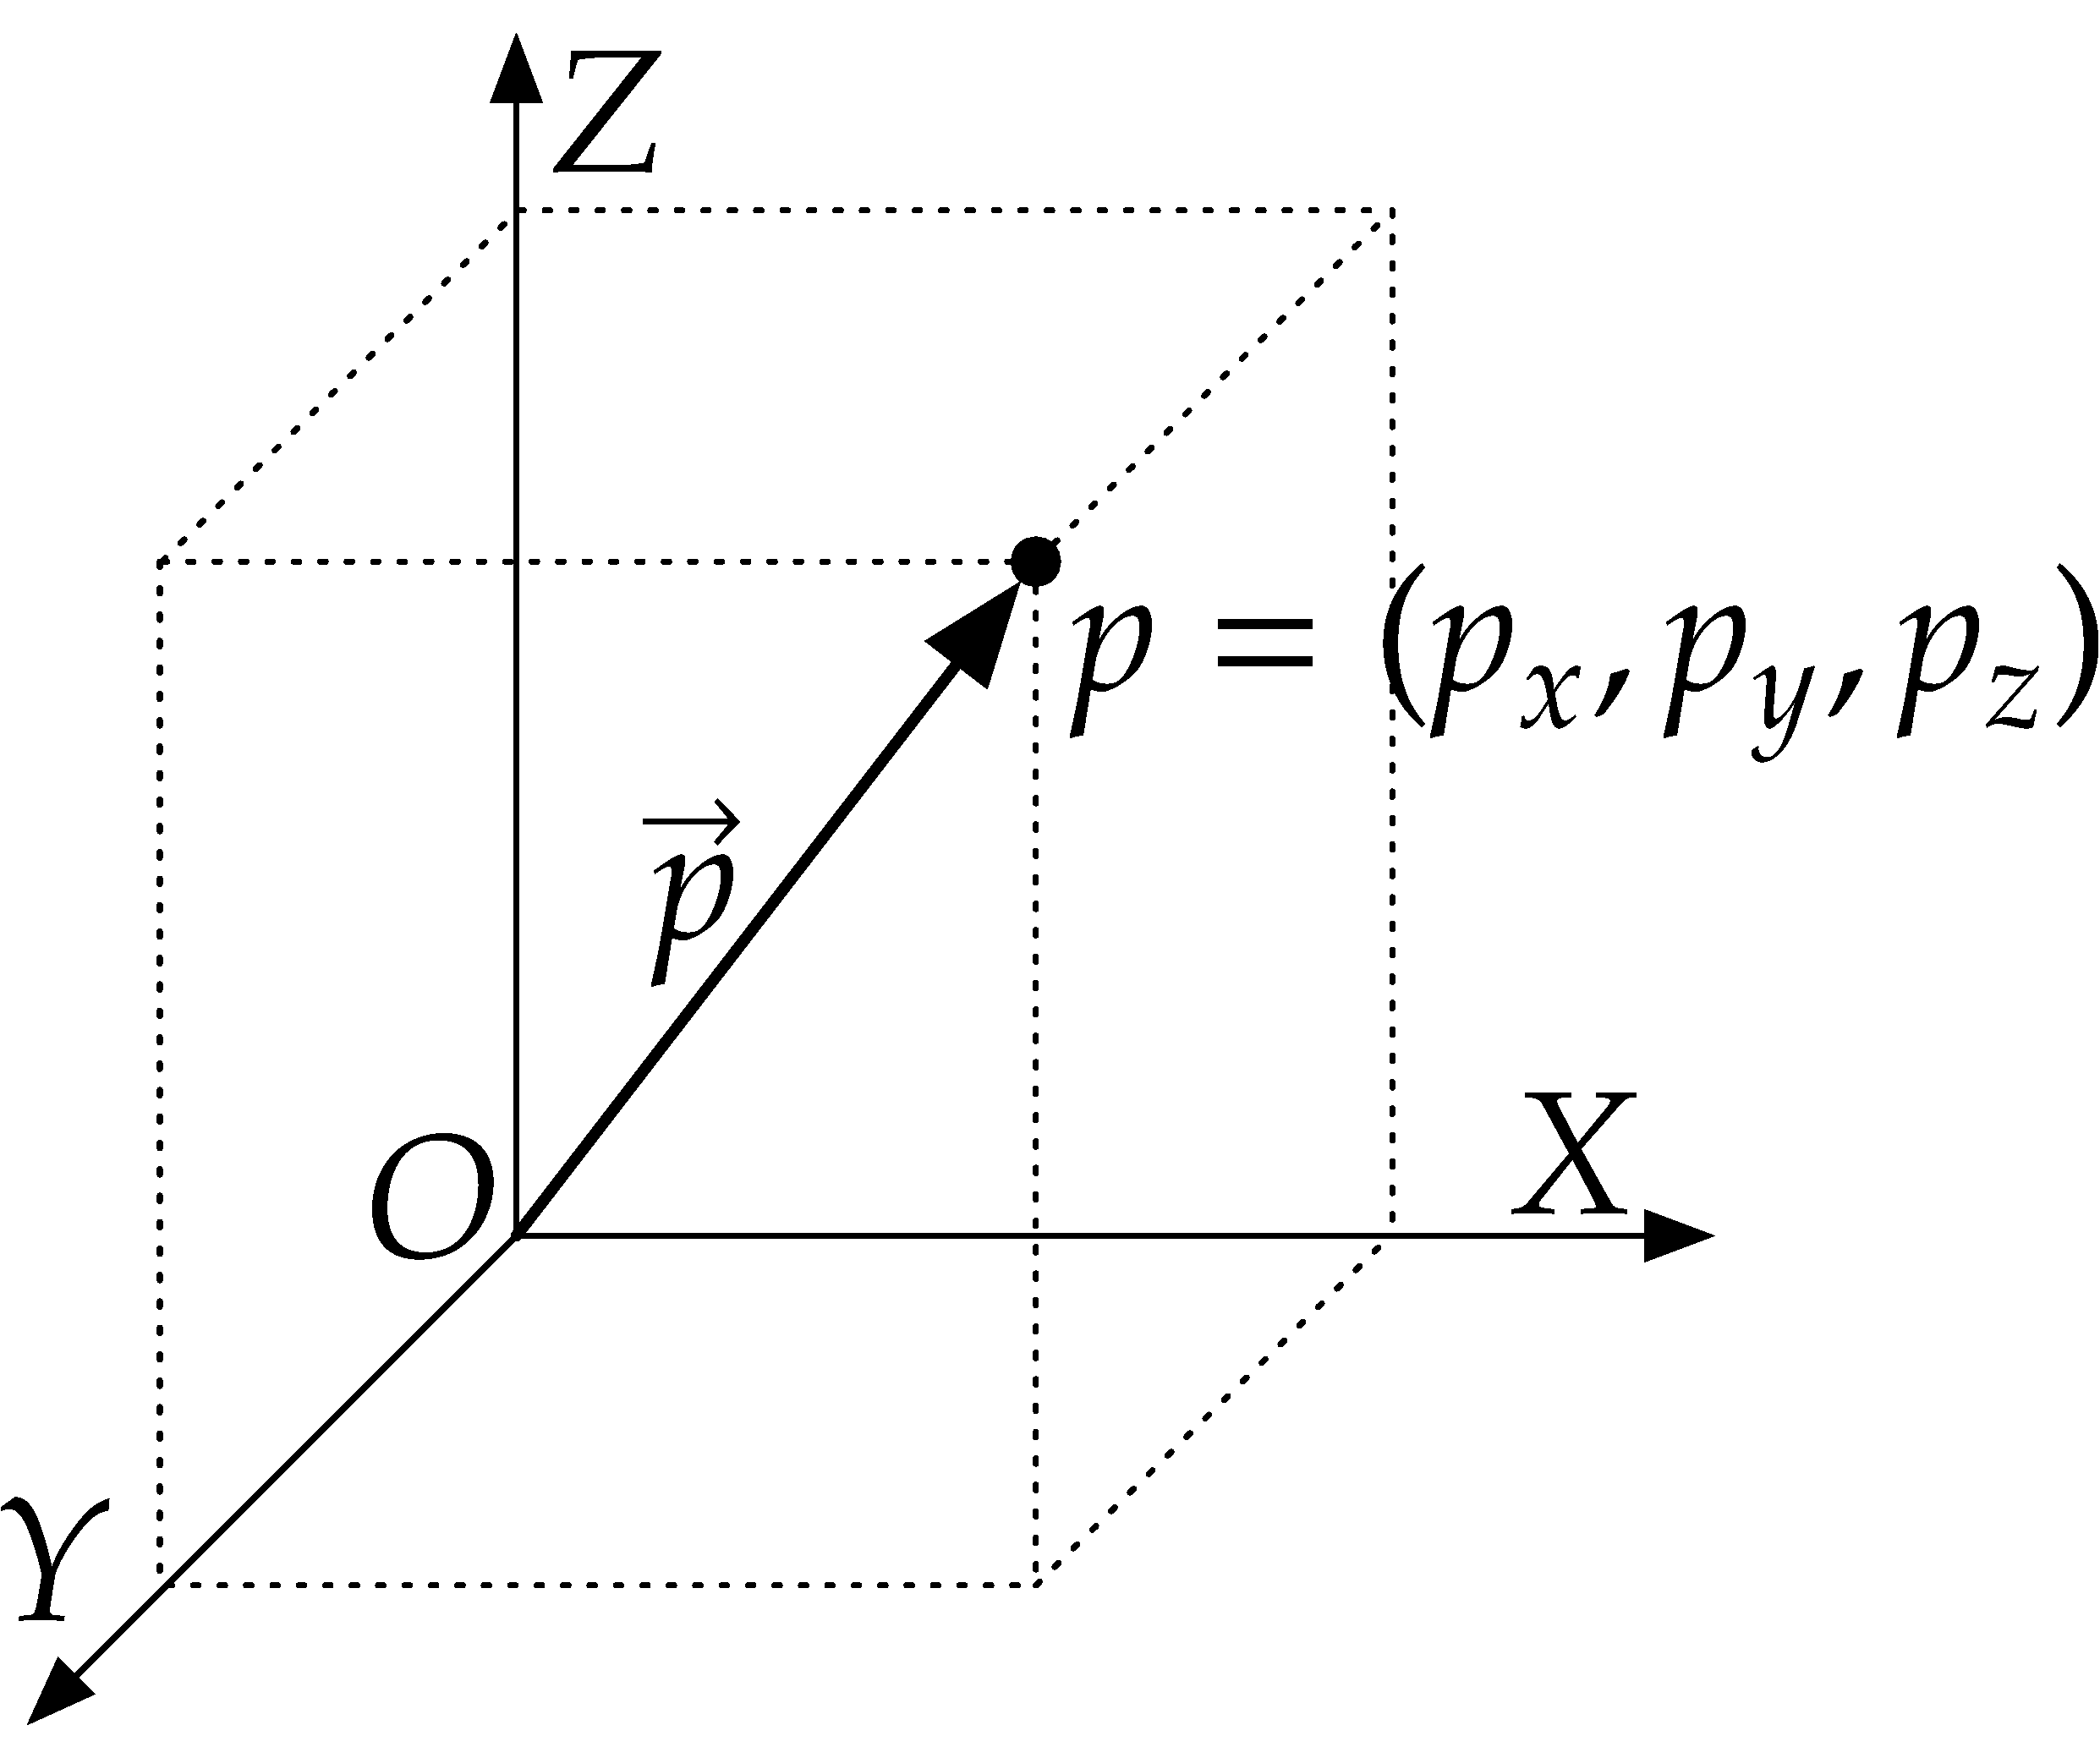
\includegraphics[width=0.3\linewidth]{figs/point.pdf}
\caption{A point in 3D described by an ordered list of three coordinates $(p_x,p_y,p_z)$.}%
\label{fig:point}
\end{figure}

Pure analytical solutions can be however tricky (\eg\ points placed at irrational values), so some other definitions used for modelling objects rely on \emph{point set geometry}.
This method uses the mathematical definitions of sets and of operations between sets to define objects as sets of (often infinitely many) points.
For instance, we can say that a sphere is a point set where the distance to a given point (\ie\ the centre) is equal to a value, or to define an object as the intersection between two other objects (\reffig{fig:boolean}).

\begin{figure}
\centering
\begin{subfigure}[b]{0.45\linewidth}
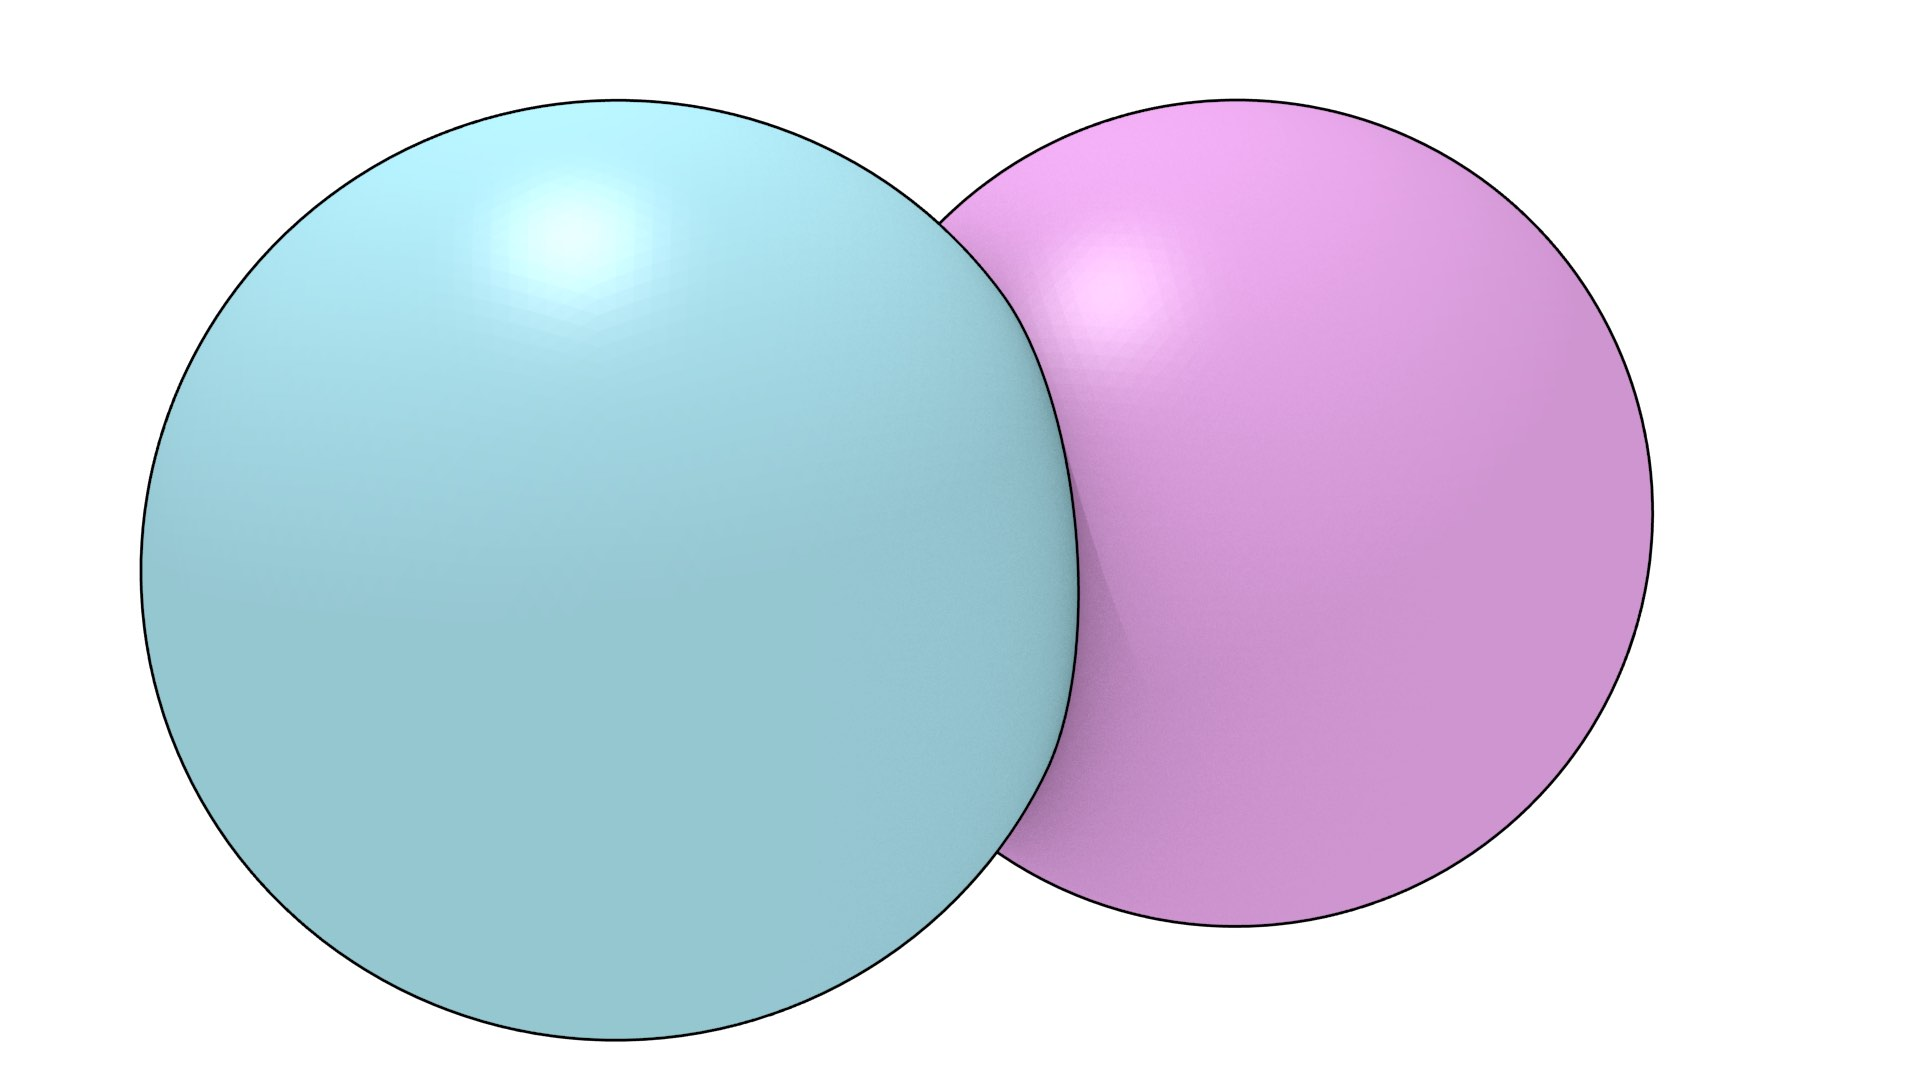
\includegraphics[width=\linewidth]{figs/boolean}
\caption{$\mathbb{A}$ (purple) and $\mathbb{B}$ (blue)}%
\label{subfig:boolean}
\end{subfigure}
\begin{subfigure}[b]{0.45\linewidth}
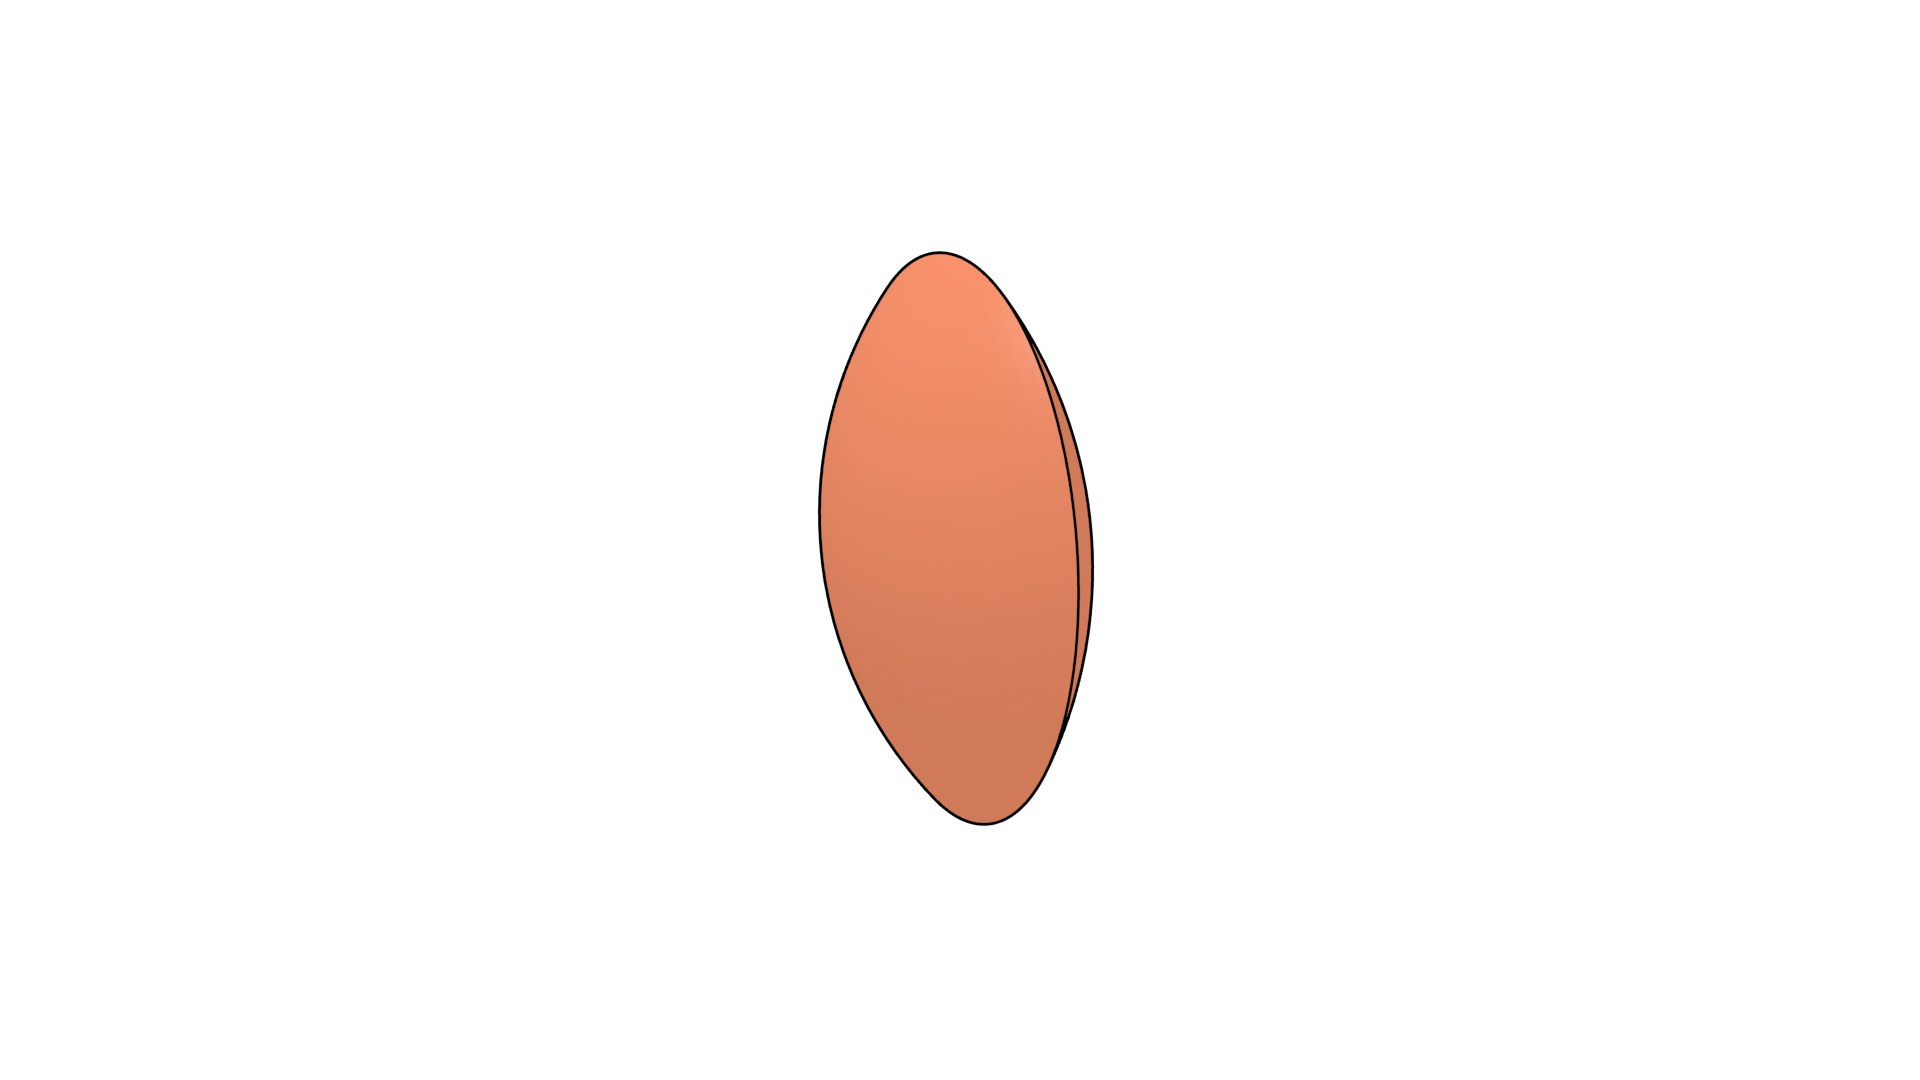
\includegraphics[width=\linewidth]{figs/boolean-intersection}
\caption{Intersection: $\mathbb{A} \cap \mathbb{B}$}%
\label{subfig:boolean-intersection}
\end{subfigure}
\caption{Based on two balls $\mathbb{A}$ and $\mathbb{B}$, other objects that can be defined using Boolean set operations using point set geometry.}%
\label{fig:boolean}
\end{figure}

\item[Graphs and algebraic topology]
The concepts from different branches of geometry are useful to describe the overall shape of objects, but in practice we often need to add concepts of topology as well.
For instance, this is often used to describe relationships between objects, such as adjacency or connectivity.
In the geometric modelling of the built environment, topology is especially important because the standard approach to model complex objects is to divide them into small elements, and thus we also need to describe how these elements are connected.

In its simplest form, topology often takes the form of a \emph{graph}, where the elements are vertices that are connected by (directed) edges.
Vertices often correspond to geometric points and edges to geometric line segments, but this is not always the case.
For instance, in a \emph{dual} representation, vertices can correspond to polygons and the edges connecting them can correspond to the connections between adjacent polygons.

\emph{Algebraic topology} takes the concept of a graph further by allowing us to use higher-dimensional objects (\eg\ faces and volumes), which will be used to describe simplices and cells in some of the data models that we will discuss later in the course.
It also makes it possible to describe objects based on sets, as well as to create operations that modify these sets.

\end{description}

\section{Data models and data structures}

In the introduction to this lesson, we mentioned that 3D modelling is done through a series of abstractions, which means that there are different levels of representations.
Within geomatics, the typical distinction that is usually made is between \emph{data models}, which are higher-level conceptual abstractions close to the way we structure the world, and \emph{data structures}, which are lower-level abstractions close to how they are implemented in a computer.
This means that there can be many possible data structures that encode the same data model, each of which is best suited for a given purpose.

Let us go through what is a data model and a data structure in more detail.
Later in the course we will use these concepts to cover particular data models and data structures.

\begin{description}

\item[Data models]

A data model is a high-level formalised way to structure information, generally using a set of abstract classes, relationships between them, and attributes to store information about them.
In the context of geomatics, these classes are often spatial representations of real-world objects.
Some aspects that are typically defined by a data model include the kind of discretisation of space that is used (\eg\ a grid) and the formal mathematical bases of the model (\eg\ describing the basic elements of a data model as tuples).
Certain data models also include formalised operations that can be performed on their defined classes.

Data models are deliberately ambiguous and far from a computer representation, and so implementing them involves various engineering decisions and can be tricky.
Moreover, without some specific encoding rules, different people will make different engineering decisions and thus likely implement a data model very differently.

The typical examples of data models used in (older) geomatics literature are the \emph{raster} and \emph{vector} data models.
These examples are historically accurate because they are clear-cut high-level descriptions that can each be implemented in a variety of ways.
For instance, rasters can be encoded by traversing them in a given order and listing the values in each cell one by one (known as exhaustive enumeration), by splitting it into successive halves of a uniform value using a $k$-d tree, or by compressing it using a Wavelet transform (\eg\ in JPEG 2000 images).

However, it is worth noting that nowadays the term data model is most often used to refer to highly complex abstractions of the real world that are suitable for a particular domain.
These can include a mixture of geometric, topological and semantic components.
Data models are often available in the form of a \emph{schema}---a descriptive document that specifies the data model in a formal manner.
Schemas are often described using UML models (\eg\ CityGML; \reffig{fig:citygml}), although using a computer-processable language (\eg\ JSON schema in CityJSON, EXPRESS in IFC, XSD in CityGML) is generally better since it allows processing the schema, such as for validation.

\begin{figure}
\centering
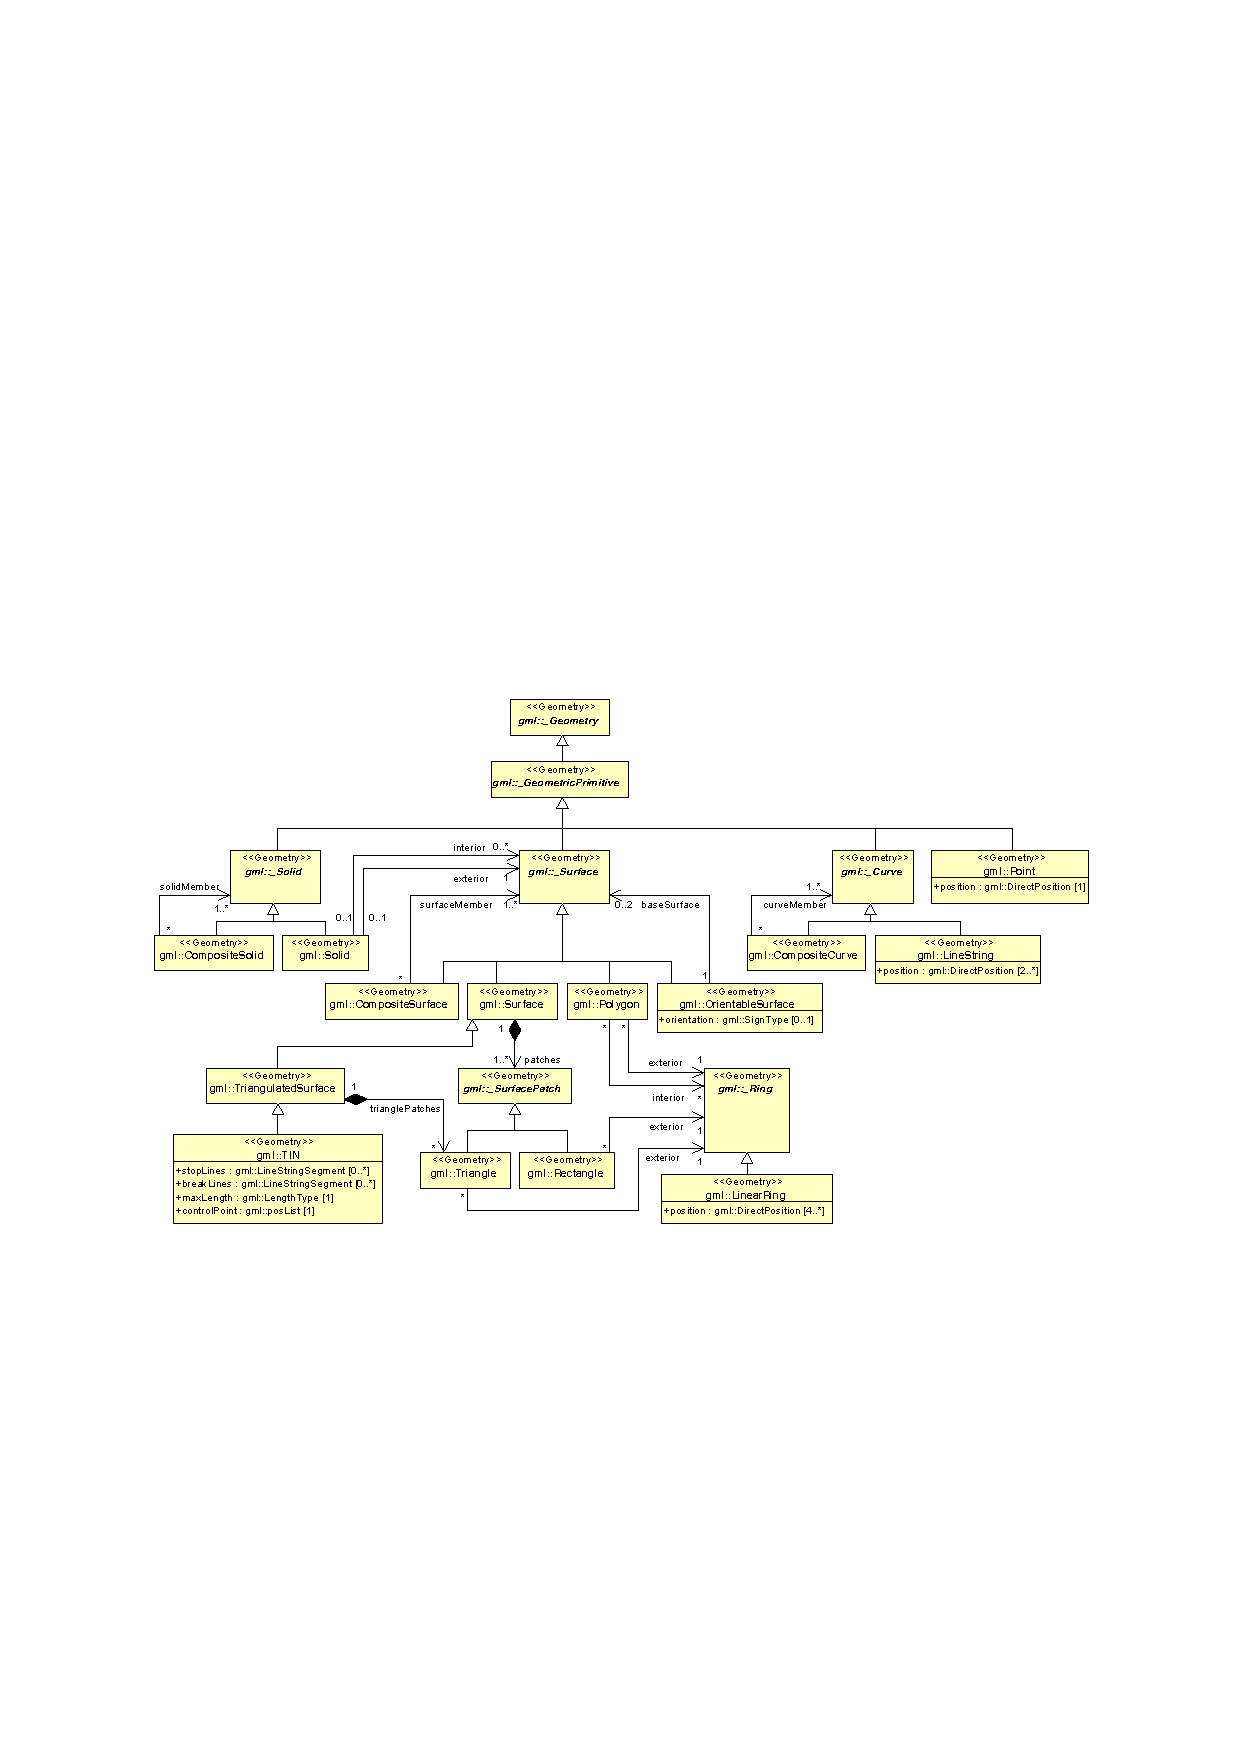
\includegraphics[width=\linewidth]{figs/citygml.pdf}
\caption{The geometry classes used in the CityGML 2.0 standard~\citep{CityGML2.0}.}%
\label{fig:citygml}
\end{figure}

\item[Data structures]

A data structure is a low-level description that specifies how to implement a data model, or occasionally a combination of multiple data models.
Data structures are defined with little to no ambiguity, specifying features such as what sort of storage should be used for a given primitive (\eg\ an array or a linked list). 
As opposed to a data model, creating a computer implementation of a data structure is thus relatively straightforward, and different people implementing the same data structure will end up with very similar implementations.

Data structures can be specified using the same methods as data models, \eg\ UML models, but more explicit descriptions are also possible.
For example, database tuples or table definitions in SQL can be used when a database implementation is expected, or snippets of source code  (generally in the style of the C programming language) can be used when it is expected to be used in memory.

Following a typical example, if we assume that we are implementing a standard vector data model with polygons, we could choose to do so using a half-edge data structure (\reffig{fig:halfedge-2}).
Note that the low-level definition of a half-edge pretty much defines the structure of its computer implementation.

\begin{figure}
\centering
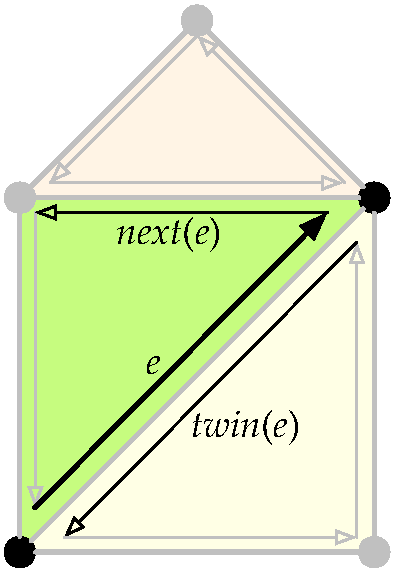
\includegraphics[width=0.3\linewidth]{figs/halfedge-2.pdf}
\caption{The half-edge data structure can store sets of polygons based on elements known as half-edges, which represent an edge within a face.
A half-edge $e$ is related to two vertices (the origin and the destination) and one face, and is linked to its next half-edge (on the same face) and its twin half-edge (on the adjacent face).}%
\label{fig:halfedge-2}
\end{figure}

\end{description}

%%%
%
\section{Exercises}

\begin{enumerate}
	\item What is noisier: the `raw' measurements in the early steps of the geoinformation chain, or the more processed products of the last steps.
	\item Consider whether a point cloud is a data model or a data structure. If it is a data model, what sort of data structure could be used to represent it?
  \item Describe an alternative data structure that can be used to represent the vector data model (\ie\ not the half-edge data structure). What are some advantages/disadvantages of each data structure?
\end{enumerate}



%%%
%
\section{Notes and comments}

\citet{Frank92} is the original source that divides representations into spatial concepts, data models and data structures.
It is partly out of date since it long predates the semantic data models that are used nowadays, but some elements match the ones we described here.

Chapter 2 of Ken's PhD thesis\footnote{\url{https://3d.bk.tudelft.nl/ken/en/thesis/math.html}} describes all the mathematical notions from this lesson in a bit more detail.
Section 3.1\footnote{\url{https://3d.bk.tudelft.nl/ken/en/thesis/modelling-background.html\#se:spatial-modelling}} lists many data models and data structures with references to the original papers where they came from.

\citet{Couclelis92} is the original source that describes the difference between objects and fields.
\citet{Goodchild92} links objects and fields to specific computer models that are suitable for them.

\citet{Mantyla88} has an excellent overview of different 3D representations.
Some other good standard alternatives are \citet{Requicha80,Hoffmann92,Foley95}.
A newer book accessible from the campus is \citet{Salomon11}.

%-------------------------------------------
%-- References
%-------------------------------------------
\bibliographystyle{../../refs/geo1004}
\bibliography{../../refs/geo1004}

\end{document}

